\FloatBarrier
\subsection{Inverted-F and center-fed monopole antenna}\label{sec:ifa_sim}

\todo[inline]{TODO}

The inverted-F antenna (IFA) and center-fed monopole antenna (CFM), shown in \crefrange{fig:center_fed_monopole}{fig:ifa}, are presented here together, because of their related geometry and similar electromagnetic behavior. Both have a maximum dimension of 5\,mm, and are electrically small at frequencies up to 6\,GHz. They exhibit an inductive nature, hence a similar behavior as the loop antenna in \autoref{sec:loop_sim} is expected. Both antennas consist of a loop of identical area to the loop antenna discussed in \cref{sec:loop_sim}, to which a linear arm is connected. In the CFM, this arm is oriented toward the TEM cell septum, whereas in the IFA it is directed toward an output port.

\begin{figure}[htbp]
	\centering
	\begin{subfigure}[b]{0.48\textwidth}
		\centering
		\includegraphics[width=0.885\textwidth]{content/img/center_fed_monopole.png}
		\caption{Geometry of CFM antenna}
		\label{fig:center_fed_monopole}
	\end{subfigure}
	\hfill
	\begin{subfigure}[b]{0.5\textwidth}
		\centering
		\includegraphics[width=1\textwidth]{content/img/inverted_f_antenna.png}
		\caption{Geometry of IFA antenna}
		\label{fig:ifa}
		\vspace{1em}
		\centering
		\includegraphics[width=1\linewidth]{content/img/cfm-ifa-moments}
		\caption{Equivalent dipole moments of IFA and CFM}
		\label{fig:cfm-ifa-moments}
	\end{subfigure}
	\caption{Geometries of IFA and CFM antenna, together with their equivalent dipole moments. the electric dipole moment $\mathbf{m}_e$ is weighted with the free space impedance $Z_0$ to enable comparison with the magnetic dipole moment $\mathbf{m}_m$.}
	\label{fig:main}
\end{figure}

%\todo[inline]{A question on my mind since the beginning of this thesis: Can how is the magnetic dipole moment influenced by rotating this geometry by 90 degrees? Is the magnetic dipole moment higher or lower than in the rotated loop antenna? With my current knowledge, I suspect that the electric dipole moment leads to current coupling with the TEM cell over displacement current, therefore leading to a smaller magnetic dipole moment then in the case of the loop antenna}

The magnetic dipole moments $\mathbf{m}_m$ of the CFM and IFA presented in \autoref{fig:cfm-ifa-moments} are comparable to each other, but are smaller in magnitude than that of the loop antenna shown in \autoref{fig:dipole_moments_loop_antenna}. This reduction can be attributed to the linear arms of the CFM and IFA, which introduce additional capacitance. The increased capacitance enhances the displacement current while reducing the induced voltage. According to \crefrange{eqn:m_v}{eqn:me_i}, this results in a decrease of magnetic dipole moment $\mathbf{m}_m$ and an increase of the electric dipole moment $\mathbf{m}_e$. 

Furthermore, for small loop and inductive antennas in general, \autoref{eqn:loop_w0} predicts that an increase in capacitance leads to a stronger non-linear frequency dependence of both $\mathbf{m}_m$ and $\mathbf{m}_e$. This assumption is confirmed by comparing the dipole moments of the loop antenna with those of the CFM and IFA, shown in \crefrange{fig:dipole_moments_loop_antenna}{fig:cfm-ifa-moments}.

\todo{CFM at 90° rotation still demonstrates magnetic dipole moment, opposed to current loop. Does this scale with antenna height, i.e. electric dipole moment?}

\FloatBarrier



%\subsubsection{Serial Loop Antenna}
%
%This section will discuss the antenna displayed in \autoref{fig:serialloopantenna}. The idea of that antenna is to create two magnetic dipole moments, which are in phase. As the frequency increases, the displacement current between the loops becomes larger, thus reducing the current through and weakening the second loop. The dipole moments in \autoref{fig:serialloopantennadipolemoments} demonstrate a non-linear behavior of the magnetic dipole moment (only very weakly recognizable, but with a geometry sweep this becomes clearer \todo{Find a geometry where this effect is much stronger}). Also, it would be interesting to measure the wave impedances in both loops over the frequency. Also, find the current distributions, add current plots and electric fields, charge distributions.  
%
%\begin{figure}[h]
%	\centering
%	\includegraphics[width=0.3\linewidth]{content/img/serial_loop_antenna}
%	\caption{Serial loop antenna}
%	\label{fig:serialloopantenna}
%\end{figure}
%\begin{figure}[h]
%	\centering
%	\includegraphics[width=1\linewidth]{content/img/serial_loop_antenna_dipole_moments}
%	\caption{Dipole moments }
%	\label{fig:serialloopantennadipolemoments}
%\end{figure}

\FloatBarrier